\section{Conceptual Model}
\label{conceptual_model}

An agent is an unit in the system capable of take independent actions. In your conceptual model an agent is an independent computational unit that manages its own resources (CPU, memory, disk, sensors, etc).

The system requirements will be represented by 'capacities'. Capacities are what goals a system can accomplish in a goal-model semantics. The system 'capacities' are implemented by 'strategies'.
The 'strategy' is both a mean of achieving a goal (as in goal-based RE) and a component in the architecture. By this we aim at creating an appropriate abstraction to allow composable adaptable architecture while keeping the traceability between the requirements and implementation at runtime.

An agent in the system has a repository of strategies that had all its runnable code. The agent have a model of that repository that it can use for reason about its capacities. The agent can also insert and remove strategies from its repository.


\begin{itemize}
  \item \textbf{Capability}: description of a kind of goal that an agent can perform.   Its an interface description in the architecture. (e.g SUM a and b)
  \item \textbf{Goal Instance}: an actual instance of an objective for a given data set. (e.g SUM 2 and 3)
  \item \textbf{Strategy}: a strategy is a 'Capability Goal' alternative implementation (e.g (SUM,a,b) => {a+b}). Its also a module in the architecture.
  \item \textbf{Strategies Resepository}: repository of know strategies
  \item \textbf{Utilitarian Function}: select strategies based on context
  \item \textbf{Runtime Context Model}: data structures that represent the knowledge of the agent.
\end{itemize}

In the proposed model an actor achieve a goal by \emph{deploing a strategy}. For instance the deployment of goals is a capability itself, as follows

\begin{itemize}
\item \textbf{<Fulfill Goals> Goal} the capability of fulfill generic goals.

\item \textbf{<Utilitarianlly Fulfill Goals> Strategy } strategy to fulfill goals by selecting available strategies and evaluating them with an utilitarian function. Consist of 3 sub-goals:
  \begin{itemize}
    \item Find Matching Strategies
    \item Decide on Strategies
    \item Deploy the Selected Strategy
  \end{itemize}
\end{itemize}

And the following three strategies implement the previous 3 goals.

\begin{itemize}
  \item \textbf{<Find Local Matching Strategies> Strategy} accomplish <find matching strategies>
  return the list of matching strategies. An matching strategy is any strategy that implement the goal interface.

  \item \textbf{<Utilitarianlly Select a Strategy> Strategy} accomplish <Utilitarianlly Fulfill Goals>
  use a pre-configured utilitarian function that analyses strategies metadata and select a strategy.

  \item \textbf{<Deploy Strategy> Strategy} accomplish <Deploy Strategy>.
  Consist of call the strategy code for the 'goal issue' runtime context model.
\end{itemize}


\begin{figure}
  \centering
  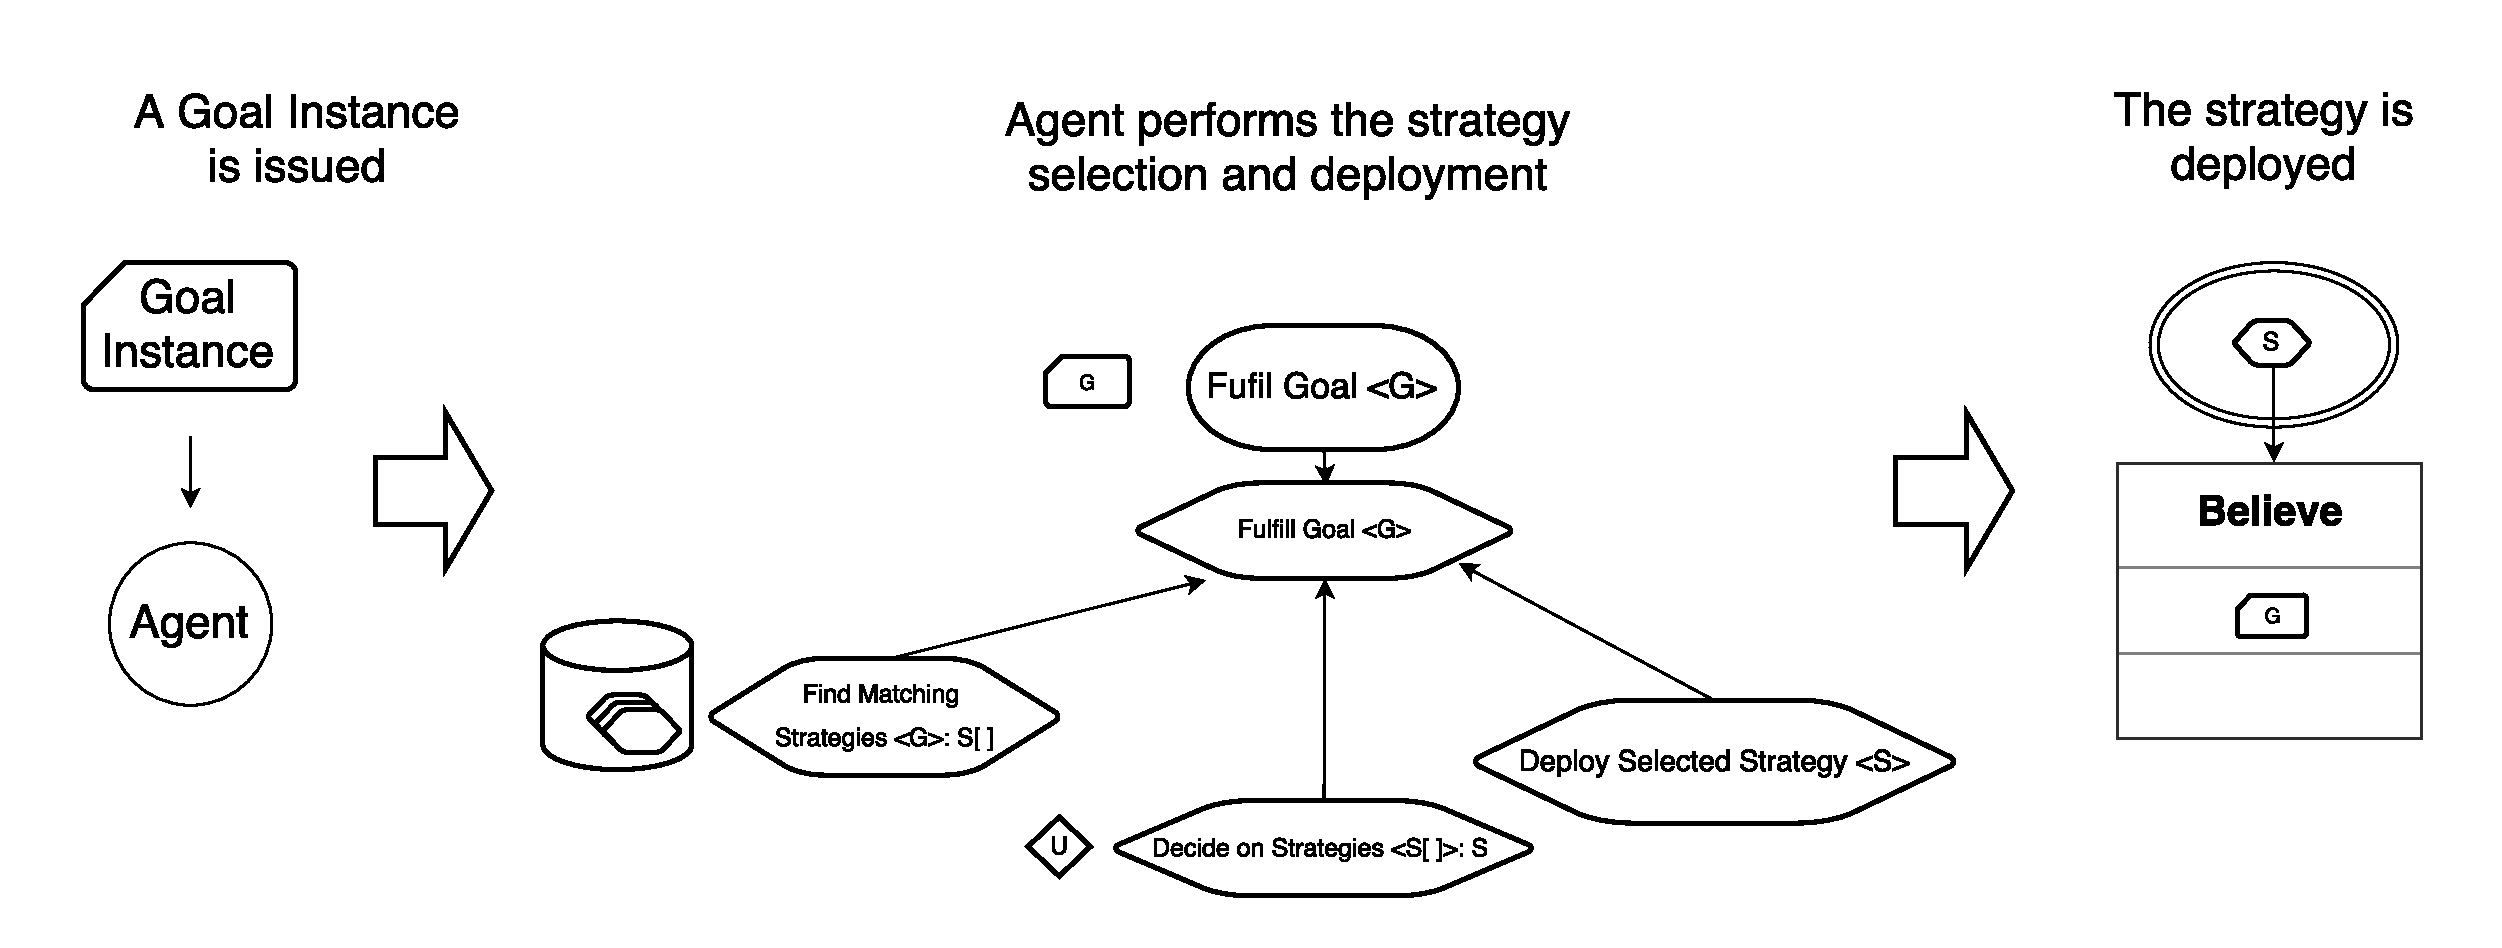
\includegraphics[width=\linewidth]{strategy_deployment}
  \caption{The deployment of a strategy}
  \label{fig:agent_composition}
\end{figure}

\section{Resources}

\section{Strategy Declaration}


\section{Fault Model}
Consistent/Inconsistent Failure

Agent failure

Resource failure

Strategy failure
